\section{OpenCV Introduction}


\centeredlargetext{white}{black}{
OpenCV Introduction
}


\begin{frame}
\frametitle{OpenCV Overview}
\begin{center}
\begin{columns}[c]
\column{0.8\textwidth}
\begin{itemize}
\item What is OpenCV?  OpenCV is \ldots
  \begin{itemize}
  \item an open source computer vision library.
  \item written in C, but has C++ and Python APIs.
  \item released under a BSD license.
  \item supported and guided by Willow Garage.
  \item found at \url{http://opencv.willowgarage.com/wiki/}.
  \end{itemize}
\end{itemize}
\column{0.2\textwidth}
 
\includegraphics[width=0.8\textwidth]{OpenCVLogo.png}
\end{columns}
\pause
\begin{itemize}
\item We will be using OpenCV 2.2 (from subversion).
\item The new C++ interface will be used when possible.
\item We assume you have some prior experience with OpenCV
\item \ldots but we will cover the basics in case you don't.
\end{itemize}
\end{center}
\end{frame}


\begin{frame}
\frametitle{Include Header Files}
\framesubtitle{OpenCVIntroduction/exercise1/BasicFilteringOpenCV.cxx}
\begin{center}
We need to include the OpenCV headers
\lstlistingwithnumber{19}{20}{BasicFilteringOpenCV.cxx}
\pause
\vspace{1 em}
and standard library headers for {\tt cout} and {\tt string}
\lstlistingwithnumber{22}{23}{BasicFilteringOpenCV.cxx}
\end{center}
\end{frame}


\begin{frame}
\frametitle{The Main function}
\framesubtitle{OpenCVIntroduction/exercise1/BasicFilteringOpenCV.cxx}
\begin{center}
\begin{itemize}
\lstlistingwithnumber{26}{52}{BasicFilteringOpenCV.cxx}
\end{itemize}
\end{center}
\end{frame}


\begin{frame}
\frametitle{Loading an Image / Applying a Filter}
\framesubtitle{OpenCVIntroduction/exercise1/BasicFilteringOpenCV.cxx}
\begin{center}
\begin{itemize}
\item If no arguments, print usage and exit \\
Note: {\tt argv[0]} contains the executable name
\lstlistingwithnumber{28}{32}{BasicFilteringOpenCV.cxx}
\pause
\item Load an image from the specified file into a matrix object
\lstlistingwithnumber{34}{34}{BasicFilteringOpenCV.cxx}
\pause
\item Create a matrix for the output and apply a median filter
\lstlistingwithnumber{35}{36}{BasicFilteringOpenCV.cxx}
\item The last argument represent the size of the filter, $9\times9$ in this case
\end{itemize}
\end{center}
\end{frame}


\begin{frame}
\frametitle{Displaying an Image}
\framesubtitle{OpenCVIntroduction/exercise1/BasicFilteringOpenCV.cxx}
\begin{center}
\begin{itemize}
\item If no output file is specified, use HighGUI to display the resulting image.
\lstlistingwithnumber{38}{45}{BasicFilteringOpenCV.cxx}
\end{itemize}
\end{center}
\end{frame}


\begin{frame}
\frametitle{Create the Display Window}
\framesubtitle{OpenCVIntroduction/exercise1/BasicFilteringOpenCV.cxx}
\begin{center}
\begin{itemize}
\item A title string is used to identify the GUI window.
\lstlistingwithnumber{40}{40}{BasicFilteringOpenCV.cxx}
\pause
\item Create a named window.
  \begin{itemize}
  \item {\tt\small CV\_WINDOW\_FREERATIO} is needed for display using OpenGL.
  \end{itemize}
\lstlistingwithnumber{41}{41}{BasicFilteringOpenCV.cxx}
\pause
\item Resize the window to match the image size.
  \begin{itemize}
  \item {\tt\small cvResizeWindow()} is a C function with no C++ API equivalent.
  \item It is not in the {\tt\small cv} namespace.
  \item It requires a {\tt\small const char*} name, provided by {\tt\small std::string::c\_str()}.
  \item The +50 in height to account for the height of tool/status bars.
  \end{itemize}
\lstlistingwithnumber{42}{42}{BasicFilteringOpenCV.cxx}
\end{itemize}
\end{center}
\end{frame}


\begin{frame}
\frametitle{Display and Wait}
\framesubtitle{OpenCVIntroduction/exercise1/BasicFilteringOpenCV.cxx}
\begin{center}
\begin{itemize}
\item Show the image in the previously created window.
\lstlistingwithnumber{43}{43}{BasicFilteringOpenCV.cxx}
\pause
\item Wait for the user to press a key, then continue.
\lstlistingwithnumber{44}{44}{BasicFilteringOpenCV.cxx}
\end{itemize}
\end{center}
\end{frame}


\begin{frame}
\frametitle{Saving an Image}
\framesubtitle{OpenCVIntroduction/exercise1/BasicFilteringOpenCV.cxx}
\begin{center}
\begin{itemize}
\item If an output file is specified, write the image to the specified file
\lstlistingwithnumber{46}{49}{BasicFilteringOpenCV.cxx}
\end{itemize}
\end{center}
\end{frame}


\begin{frame}[fragile]
\frametitle{Exercise 1}
\framesubtitle{OpenCVIntroduction/exercise1/BasicFilteringOpenCV.cxx}
\begin{center}
\begin{itemize}
\item Replace the median filter with a Canny edge detector
\lstlistingwithnumber{35}{36}{BasicFilteringOpenCV.cxx}
\pause
\item Hint: The OpenCV Canny function has this signature
\begin{lstlisting}[numbers=none,xleftmargin=0pt]
void Canny(const Mat& image, Mat& edges, double threshold1, double threshold2);
\end{lstlisting}
\pause
\item Canny requires grayscale image input, but our images are color
\item Hint: Use this function to convert a color space
\begin{lstlisting}[numbers=none,xleftmargin=0pt]
void cvtColor(const Mat& src, Mat& dst, int code);
\end{lstlisting}
\item Use {\tt CV\_BGR2GRAY} for {\tt code} to convert BGR color to gray.
\end{itemize}
\end{center}
\end{frame}


\begin{frame}
\frametitle{Exercise 1: Answer}
\framesubtitle{OpenCVIntroduction/exercise1/BasicFilteringOpenCVAnswer.cxx}
\begin{center}
\begin{itemize}
\lstlistingwithnumber{34}{38}{BasicFilteringOpenCVAnswer.cxx}
\end{itemize}
\begin{columns}[c]
\column{0.5\textwidth}
\begin{center}
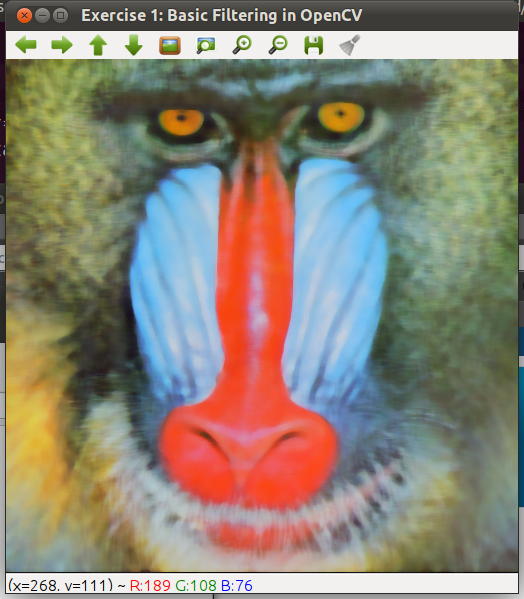
\includegraphics[width=0.5\textwidth]{OpenCVex1-GUI.png} \\
Median Filter
\end{center}
\column{0.5\textwidth}
\begin{center}
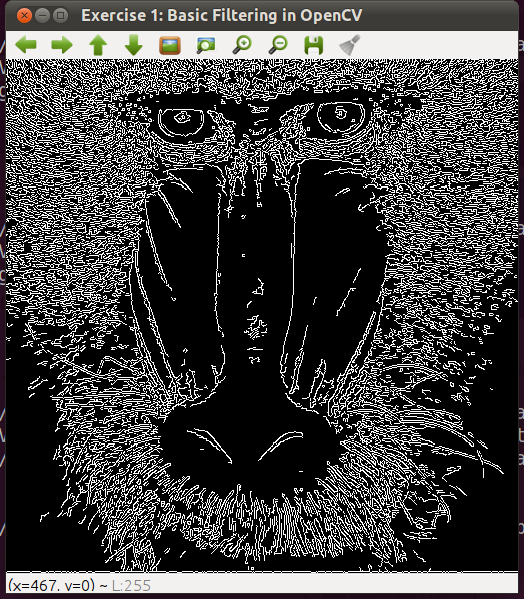
\includegraphics[width=0.5\textwidth]{OpenCVex1-ans-GUI.png} \\
Canny Edges
\end{center}
\end{columns}
\end{center}
\end{frame}


\begin{frame}
\frametitle{Exercise 2: Basic Video Filtering}
\framesubtitle{OpenCVIntroduction/exercise2/BasicVideoFilteringOpenCV.cxx}
\begin{center}
\begin{itemize}
\item Video filtering is similar to image filtering, except
  \begin{itemize}
  \item use a {\tt VideoCapture} object to read a video file.
  \item loop over each frame in the video and process each one.
  \item display or encode each output frame within the loop.
  \end{itemize}
\end{itemize}
\end{center}
\end{frame}


\begin{frame}
\frametitle{Loading a Video File}
\framesubtitle{OpenCVIntroduction/exercise2/BasicVideoFilteringOpenCV.cxx}
\begin{center}
\begin{itemize}
\item The first step is to open the video file and parse the headers.
\lstlistingwithnumber{88}{93}{BasicVideoFilteringOpenCV.cxx}
\item If unable to parse the headers then terminate the program.
\end{itemize}
\end{center}
\end{frame}


\begin{frame}
\frametitle{Display or Save}
\framesubtitle{OpenCVIntroduction/exercise2/BasicVideoFilteringOpenCV.cxx}
\begin{center}
\begin{itemize}
\item Same command line usage as before for selecting between displaying
      or saving results.
\item The processing code has been encapsulated into functions.
\item If only input video is specified, then display the resulting video.
\lstlistingwithnumber{95}{98}{BasicVideoFilteringOpenCV.cxx}
\item If a second file is specified, then save the resulting video to the file.
\lstlistingwithnumber{99}{102}{BasicVideoFilteringOpenCV.cxx}
\end{itemize}
\end{center}
\end{frame}


\begin{frame}
\frametitle{Prepare the Display Window}
\framesubtitle{OpenCVIntroduction/exercise2/BasicVideoFilteringOpenCV.cxx}
\begin{center}
\begin{itemize}
\item This function processes the video and displays the results.
\lstlistingwithnumber{35}{36}{BasicVideoFilteringOpenCV.cxx}
\pause
\item Use the {\tt\small get()} member function to access video properties: \\
      frame rate, width, and height.
\lstlistingwithnumber{37}{39}{BasicVideoFilteringOpenCV.cxx}
\pause
\item Setup the HighGUI window as in the previous example.
\lstlistingwithnumber{41}{43}{BasicVideoFilteringOpenCV.cxx}
\end{itemize}
\end{center}
\end{frame}


\begin{frame}
\frametitle{Process and Display}
\framesubtitle{OpenCVIntroduction/exercise2/BasicVideoFilteringOpenCV.cxx}
\begin{center}
\begin{itemize}
\item Number of milliseconds to wait before drawing the next frame.
\lstlistingwithnumber{45}{45}{BasicVideoFilteringOpenCV.cxx}
\pause
\item Loop until no more frames can be read from the video capture object.
\lstlistingwithnumber{47}{57}{BasicVideoFilteringOpenCV.cxx}
\item Call {\tt\small processFrame()} on each frame and and display the result.
\item {\tt waitkey(\emph{delay})} returns positive value indicating the key pressed
      or returns -1 after {\tt \emph{delay}} ms have passed.
\end{itemize}
\end{center}
\end{frame}


\begin{frame}
\frametitle{Create a Video Writer}
\framesubtitle{OpenCVIntroduction/exercise2/BasicVideoFilteringOpenCV.cxx}
\begin{center}
\begin{itemize}
\item This function processes the video and saves the results.
\lstlistingwithnumber{62}{63}{BasicVideoFilteringOpenCV.cxx}
\pause
\item Get the video properties as before.
\lstlistingwithnumber{64}{66}{BasicVideoFilteringOpenCV.cxx}
\pause
\item Specify that the output video will be encoded in DIVX format.
\item Create a video writer object with the specified filename.
\lstlistingwithnumber{68}{70}{BasicVideoFilteringOpenCV.cxx}
\end{itemize}
\end{center}
\end{frame}


\begin{frame}
\frametitle{Process and Save}
\framesubtitle{OpenCVIntroduction/exercise2/BasicVideoFilteringOpenCV.cxx}
\begin{center}
\begin{itemize}
\item Loop until no more frames can be read from the video capture object.
\lstlistingwithnumber{71}{76}{BasicVideoFilteringOpenCV.cxx}
\item Call {\tt\small processFrame()} on each frame.
\item Write the resulting image to the output video file with the insertion operator ({\tt\small <<}).
\end{itemize}
\end{center}
\end{frame}


\begin{frame}
\frametitle{Exercise 2}
\framesubtitle{OpenCVIntroduction/exercise2/BasicVideoFilteringOpenCV.cxx}
\begin{center}
\begin{itemize}
\item Implement {\tt\small processFrame()} by adding the Canny edge detector.
\lstlistingwithnumber{27}{31}{BasicVideoFilteringOpenCV.cxx}
\pause
\item Saving to a video requires color images, but Canny produces grayscale images.
\item Hint: Use {\tt\small cvtColor()} again to convert back to color.
\item Use code {\tt\small CV\_GRAY2BGR} for {\tt\small code} to convert gray to BGR.
\end{itemize}
\end{center}
\end{frame}
